\section{Primary dataset overview} % A representative dataset for ping latency analysis}
\label{sec:dataset}

In this section, we describe the ISI survey dataset we use for our
analysis of ping latency. We perform a preliminary analysis of ping
latency and find that the dataset contains different types of
responses that should (or should not) be matched to identify
high-latency responses. Finally, we describe techniques to remove
responses that could induce errors in the latency analysis.


\subsection{Raw ISI survey data}

ISI has conducted Internet wide
surveys~\cite{census-survey} since 2006.  Precise
details can be found in Heidemann et
al.~\cite{census-survey}, and technical details
of the data format online~\cite{isi-survey-binformat}, but we present a brief
overview here.

Each survey includes pings sent to approximately 24,000 /24
address blocks, meant to represent 1\% of all allocated IPv4
address space.  Once an address block is included, ICMP echo
request probes are sent to all 256 addresses in the selected
/24 address blocks once every 11 minutes, typically for two
weeks.  The blocks included in each survey consist of four
classes, including blocks that were chosen in 2006 and
probed ever since, as well as samples of blocks that were
responsive in the last census---another ISI project that probes
the entire address space, but less frequently.  However, we treat the union of
these classes together.

We use data from 103 surveys taken between April 2006 and
February 2015, and performed initial studies based on 2011--2013 data, but focus on the most recent of them, in January and February of 2015 for data quality and timeliness.  
The dataset consists of all echo requests
that were sent as part of the surveys in this period, as
well as all echo responses that were received.  Of
particular importance is that echo responses received
within, typically, three seconds of an echo request to the
same address are matched into a single record and given a
round-trip measurement precise to microseconds.  Should an
echo response take four seconds to arrive, a ``timeout''
record is recorded associated with the probe, and an
``unmatched'' record is recorded associated with the
response.  These two packets have timestamps precise only to
seconds.  The dataset also includes ICMP error responses
(e.g., ``host unreachable''); we ignore all probes
associated with such responses since the latency of ICMP error
responses is not relevant.

In later sections, we will complement this dataset with
results from Zmap~\cite{durumeric2013zmap} and additional experiments
including more frequent probing with Scamper~\cite{luckie2010scamper} and
Scriptroute~\cite{usits03-spring}.

\subsection{Matched response latencies are capped at the timeout}

\begin{figure}[tb]
\begin{center}
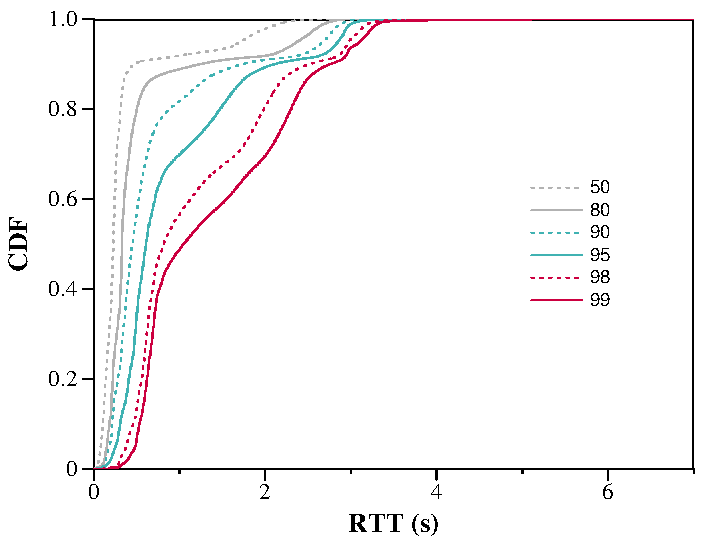
\includegraphics[width=3in]{timeouts/figs/cdf_raw_ping_ttl}
\end{center}
\caption{\label{fig:raw_lat}%
CDF of percentile latency of survey-detected responses per IP address: Each point represents an IP address
and each curve represents the percentile from that IP address's
response latencies. The slope of the latency
percentiles increases around the 3 second mark, suggesting that
ISI's prober timed out responses that arrived after 3 seconds.
}
\end{figure}

In this section, we present the latencies we would observe
when considering only those responses that were matched to 
requests because they arrived within the timeout.  We call 
these responses \emph{survey-detected responses}.

We aggregate round trip time measurements in terms of the
distribution of latency values per IP address, focusing on
characteristic values on the median, 80th, 90th, 95th, 98th
and 99th percentile latencies.  That is, we attempt to treat
each IP address equally, rather than treat each ping
measurement equally.  This aggregation ensures that
well-connected hosts that reply reliably are not
over-represented relative to hosts that reply infrequently.

Taking ISI survey datasets from 2011--2013 together, we show a CDF of
these percentile values considering only survey-detected
responses in Figure~\ref{fig:raw_lat}.  Taken literally, 95\%
of echo replies from 95\% of addresses will arrive in less than
2.85 seconds.  However, it is apparent that the distribution
is clipped at the 3 second mark, although a few responses
were matched even after 7 seconds.   

We observe three broad phases in this graph: (1) the lower
40\% of addresses show a reasonably tight distribution in
which the 99th percentile stays close to the 98th; (2) the
next 50\% in which the median remains low but the higher
percentiles increase; and (3) the top 10\% where the median
rises above 0.5 seconds.


\subsection{Unmatched responses}

If a probe takes more than three seconds to solicit a
response, it appears as if the probe timed-out and the
response was unsolicited or \emph{unmatched}.  Since it
appears from Figure~\ref{fig:raw_lat} that three seconds is
short enough that it is altering the distribution of round
trip times, we are interested in matching these echo
responses to construct the complete distribution of round
trip times.

Matching these responses to find \emph{delayed responses} is
not a simple matter, however.  In particular, we find two
causes of \emph{unexpected responses} that should not yield
samples of round trip times: unmatched responses solicited
by echo requests sent to broadcast addresses and apparent
denial of service responses.

% We require the union of low-rtt responses' latencies and high-rtt
% responses' latencies to perform an analysis of ping
% latencies. 
% \subsection{Matching delayed responses}

We match a delayed response with its corresponding request
as follows: Given an unmatched response having a source IP
address, we look for the last request sent to that IP
address.  If the last request timed out and has not been matched, the latency is then the difference between the
timestamp of the response and the timestamp of the
request.  ISI recorded the timestamp of unmatched responses
to a 1 second precision, thus the latencies of inferred
delayed responses are precise only to a second.

The presence of unexpected responses can lead to the
inference of incorrect latencies for delayed responses using
this technique: not all unexpected responses should be
matched by source address.
We thus develop filters to remove unexpected responses from the set of
unmatched responses.

We note that it is possible to match responses to requests
explicitly using the id and sequence numbers associated with
ICMP echo requests, and even perhaps using the payload.
These attributes were not recorded in the ISI dataset, which
motivates us to develop the source address based scheme.  We
use these fields when running Zmap or other tools to confirm
high latencies in Section~\ref{sec:verification} below.


% Some of
% these unmatched responses are higher latency responses which arrived
% at the prober after the timeout duration; we call these responses high-rtt
% responses. The remaining unmatched responses are unexpected responses, sent either
% in response to an echo request addressed to a broadcast address or as part
% of a Denial of Service attack. 

% \subsection{Unexpected Responses}
% 
% The dataset contains two sources of unexpected responses: Responses
% obtained from probes sent to broadcast addresses and
% duplicate responses.  We discuss each in turn. 
% Our goal is to study the latency of pings, including both low-rtt as
% well as high-rtt responses. To recover high-rtt responses from the
% data, we need to match unmatched echo Responses with their corresponding echo Requests.

% Have a figure here which shows the distribution of latencies from the
% raw pings, and how we found out that it has a 3 second timeout.
% ISI has a timeout of 3 seconds. Drop everything that arrives after
% then.

% When we tried reconstructing, we had to clean up a bunch. Had the
% following problems:

\subsubsection{Broadcast responses}

% We show that several unmatched responses are caused by
The dataset contains several instances where a ping to a
destination times out, but is closely followed by an
unmatched response from a source address that is within the same /24
address block, but different from the destination.
% The dataset contains several unmatched
% responses that were received immediately after a ping was sent to a different
% address within the same /24 address block.
In each round of probing, this behavior repeats.
%
Here, we analyze these unmatched responses, find that they are likely
caused by probing broadcast addresses, and filter them.

Network prefixes often include a broadcast address, where one
address within a subnet represents all devices connected to
that prefix~\cite{rfc919}.
%
The broadcast address in a network should
be an address that is
unlikely to be assigned to a real host~\cite{rfc919}, such as the
address whose host-part bits are all 1s or 0s, allowing us to
characterize broadcast addresses.
%
Devices that receive an echo
request sent to the broadcast address may, depending on
configuration, send a response~\cite{rfc1122}, and if sending a response,
will use a source address that is their own.
%
We call these
responses \emph{broadcast responses}.  
%
No device should send
an echo response with the source address that is the
broadcast destination of the echo request. 

% We investigate Echo Requests to destination addresses that trigger
% Echo Response from different addresses within the same /24 address blocks.
% We seek to understand why an Echo Request sent to a destination
% address would trigger an Echo Response from a different address within
% the same /24 address block.
% We hypothesize that a ping sent to broadcast address triggers
% responses from address(es) within the same /24 address block.
We hypothesize that pings that trigger responses from different
addresses within the same /24 address block result when the
ping destination is a broadcast address. 
We examine ping destinations
that solicit a response from a different address in the same /24
address block, and check if they appear to be broadcast addresses.
%
%
% These addresses will have last octets that
% can be represented as $2^n-1$ such as 63, 127, 255 etc.
%
% We wondered if network operators are following this convention.
%

We extended the ICMP probing module in the
Zmap scanner~\cite{durumeric2013zmap} to embed the destination
into the echo request, then to extract the destination from the
echo response.
%
Doing so allows us to infer the destination address to which the probe
was originally sent.
%
% We mark such a response as a
% broadcast response.
%
Zmap collected the data and made
it available for download at \url{scans.io}.
%

We choose the Zmap scan conducted closest in
time to the last ISI survey we studied, on April 17 2015, to investigate
the host-part bits of destination addresses that triggered responses
from a different address from the same /24 address block.
%
We plot the distribution of the last octets of these addresses in
Figure~\ref{fig:zmap_last_octet_hist}.
%
Last octets with the last N bits ending in 1 or 0, where N is greater than 1,
such as 255, 0, 127, 128 etc., have spikes. These addresses are likely broadcast addresses.
% Last octets with the last N bits as 1 (where N $>$ 1), such as 255, 127, etc., have the largest
% spikes. Last octets with the last N bits as 0, such as 0, 128, etc.,
% also have spikes, but smaller.
On the other hand, last octets that
end in binary '01' or '10' have very few addresses.

\begin{figure}[tb]
\begin{center}
\includegraphics[width=3in]{timeouts/figs/zmap_last_octet_hist_all_bcast_addrs_apr_17}
\end{center}
\caption{\label{fig:zmap_last_octet_hist}%
Broadcast addresses that solicit responses in Zmap: Broadcast addresses usually
have last octets whose last N bits are either 1 or 0
(where N $>$ 1).
}
\end{figure}


\subsubsection*{Broadcast responses exist in the dataset}

% Next, we show the existence of broadcast responses in the ISI dataset.
% We examine how many of the unmatched responses in the dataset are
% broadcast responses. 
%
\begin{figure}[tb]
\begin{center}
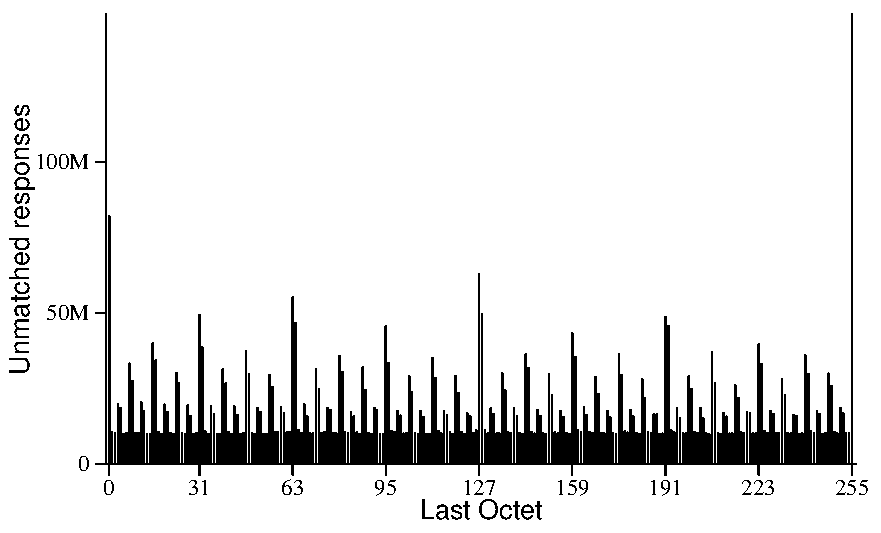
\includegraphics[width=.99\linewidth]{timeouts/figs/last_octet_hist}
\end{center}
\caption{\label{fig:bcast_hist}%
Number of unmatched responses that followed a probe sent to address
with last octet X. Last octets with last N bits ending in
0s and 1s (where N $>$ 1) observe spikes, likely caused by broadcast
responses. Not all unmatched responses are caused by broadcast
responses, however, since there exist roughly 10M unmatched
responses distributed evenly across all last octets.}
\end{figure}



We examine if unmatched responses in the ISI dataset are caused by pings sent to broadcast addresses.
%
Since broadcast responses are likely to be seen after an
Echo Request sent to a broadcast address, we find
the most recently probed address within the same /24 prefix for each
unmatched response. 
%
We then extract the last octet of the most recently probed
address.
%
Figure~\ref{fig:bcast_hist} shows the
distribution of unmatched responses across these last octets. 
%
We find that around 10M unmatched responses are distributed evenly
across all last octets: these are unmatched responses that don't seem
to be broadcast responses.
%
However, last octets that have their last N bits as 1s and 0s
,when N is greater than 1, observe spikes similar to those in Figure~\ref{fig:zmap_last_octet_hist}.
% , supporting our hypothesis that these are
% responses to broadcast addresses.
%
% These are the addresses most likely to see an
% unmatched response after an echo request to them times
% out. 
%

If left in the data, broadcast responses could yield
substantial latency overestimates in the following, common,
scenario, which we illustrate in
Figure~\ref{fig:bcast_sample}.
%
Assume that the echo request
sent to an address 211.4.10.254 is lost and that the
device is configured to respond to broadcast pings.  
%
The
echo request sent to 211.4.10.254 could then be matched to
the response to the request sent to 211.4.10.255, the
broadcast address of the enclosing prefix.  
%
This would lead
to a latency based on the interval between probing
211.4.10.254 and 211.4.10.255, as shown in the figure.

\begin{figure}[tb]
\begin{center}
% \centering
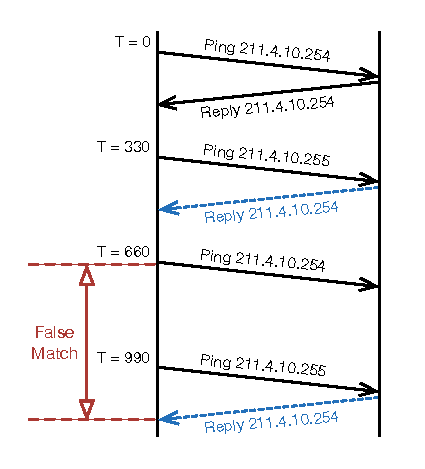
\includegraphics[width=0.97\linewidth]{timeouts/figs/wfall_bcast}
\end{center}
\caption{\label{fig:bcast_sample}%
We filter broadcast responses since they can lead to the inference of
false latencies. This figure illustrates a potential incorrect match
caused by a broadcast response.
Echo requests sent to the broadcast address 211.4.10.255 at T = 330
and T = 990 seconds solicit responses from 211.4.10.254.  When a timeout occurs 
for a request sent directly to 211.4.10.254 at T = 660 seconds, we 
would falsely connect that request to the response at T = 990 seconds.}
\end{figure}

%
% A last octet of 255 and 0 have particularly large spikes, 
% corresponding to the possible broadcast addresses of a /24 subnet.

\subsubsection*{Filtering broadcast responses}

% A potential approach to filtering broadcast responses is to check
% if an unmatched response was preceded by a ping to an address
% whose last octet had its last N bits as 1s or 0s (where N $>$ 1).
% %
% However, this scheme would have been too aggressive, potentially filtering
% delayed responses that coincidentally happened to arrive after an Echo
% Request to a broadcast address.
% %
% Thus, we develop an alternate method which uses ISI's non-random probing
% scheme to detect addresses that source broadcast responses.
%
We develop a method which uses ISI's non-random probing
scheme to detect addresses that source broadcast responses.
We call such addresses \emph{broadcast responders}, and seek to filter
all their responses.
 % and the assumption that broadcast responses, like typical Echo
% responses, have stable latencies.
%
We believe that delayed responses are likely to
exhibit high variance in their response latencies, since congestion varies over
time. 
%
On the other hand, a
broadcast response is likely to have relatively stable latency.
%
% (unless it happens to be congested too.)

ISI's probing scheme sends
probes to each address in a /24 address block in a nonrandom sequence,
allowing us to develop a filter that checks if a source address responds
to a broadcast address each round.
%
% The last octet of the probed IP address generally has its $n$th
% bit (counting from 0) swapped every $2^n$ probes on the /24 block.
Addresses are probed such that last octets that are off by one, such
as 254 and 255, receive pings spaced 330 seconds apart (half the
probing interval of 11 minutes) as shown in Figure~\ref{fig:bcast_sample}.
% nth most significant bit probed, i.e., probes to 1 and 129 are sent
% one after the other.
%
% We filter broadcast responses by looking for unmatched responses from
% the same source address that
% repeat periodically with similar latency.
%
For every unmatched response with a latency of at least 10 seconds,
the filter checks if the same source address had sent an unmatched
response with a similar latency in the previous round.
% checks whether they occurred right before another response of a
% similar latency (within 2 seconds).
%
We take an exponentially weighted moving average of the number of times
this occurs for a given source address with $\alpha=0.01$.
%
Most broadcast responders have the
maximum of this moving average $>$ 0.9, but since probe-loss can
potentially decrease this value, we mark IP addresses with values $>$
0.2 and filter all their responses. 
%
% If the maximum of this moving average per source address is greater than 0.2, the IP address
% is marked as one that responds to probes to broadcast addresses, and
% it is filtered out.
% %
% This filter is meant to be selective for the specific pattern of responses, without being so
% selective that it fails to classify broadcast addresses in the
% presence of loss.

We confirm that we find broadcast responders correctly in the
ISI surveys by comparing the ones we found in the ISI 2015 surveys
with broadcast responders from the Zmap dataset.
%
% Ideally, the Zmap scan should have been conducted at the same time as
% the ISI surveys, but we choose the closest available Zmap scan in time,
% bearing in mind that broadcast responders may change over time.
%
% The IT63w (20150117)
% and IT63c (20150206) datasets recorded responses from 4,008,830
% addresses.
% %
% The filter detected 9,942 broadcast responders among them.
%
% 8729 of these broadcast responders appeared as the source addresses
% of an Echo Response in Zmap's
% April 17 2015 scan. 
%
Zmap detected 939,559 broadcast responders in the April 17
2015 scan, of which 7212 had been
addresses that provided Echo Responses in ISI's IT63w (20150117) and
IT63c (20150206) datasets.
%
The filter detected 7044 (97.7\%) of these as broadcast responders. 
% We inspected the remaining 168 addresses and found that 159 could not have been broadcast responders at the time they were probed by ISI: their 99th percentile RTTs were far too low.
We inspected the 168 remaining addresses and found that 154 addresses
have 99th percentile latencies below 2.5 seconds. Since ISI
probes a /24 prefix only once every 2.5 seconds, these addresses
cannot be broadcast responders. Another 5 addresses have 99th
percentiles latencies below 5 seconds; these are unlikely to be
broadcast responders as well.

The remaining 9 addresses had 99th percentile latencies in excess of
300s and seem to be broadcast responders. Upon closer inspection, we
found that these addresses only occasionally sent an unmatched
response: around once every 50 rounds. The $\alpha$ parameter of the
filter can tolerate some rounds with missing responses, but these
addresses respond in so few rounds that they pass undetected. 
If these 9 are indeed broadcast responders as suggested by high 99th percentile latencies, this yields a false negative rate of our filter of 0.13\%.
% demonstrating that it is able to find broadcast responders with high
% accuracy.

\subsubsection{Duplicate responses}

Packets can be duplicated.  A duplicated packet will not affect inferred latencies as
long as the original response to the original probe packet reaches the prober, since our scheme
ignores subsequent duplicate responses. However, we find that some IP
addresses respond many times to a single probe. In this case, the incoming packets aren't responses to
probes, but are either caused by incorrect configurations or malicious
behavior. 

\begin{figure}[tb]
\begin{center}
% \centering
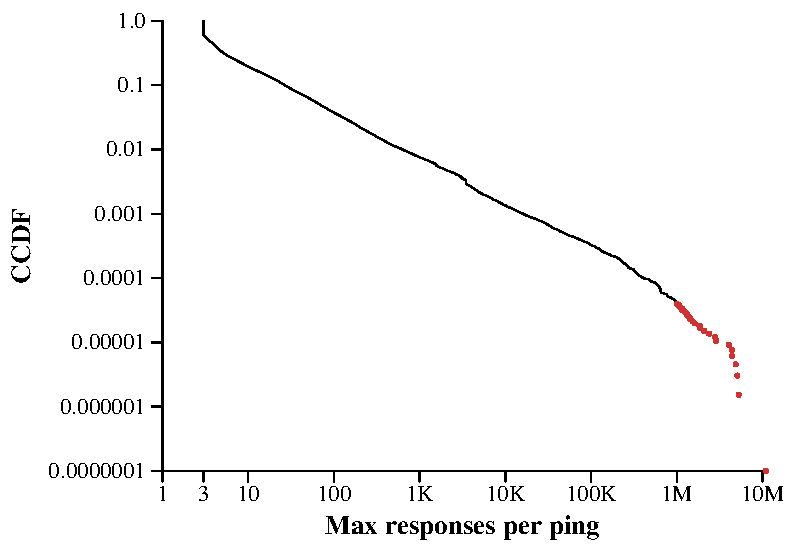
\includegraphics[width=.9\linewidth]{timeouts/figs/ccdf_dos}
\end{center}
\caption{\label{fig:dos}%
Maximum number of responses received for a single echo request, for IP
addresses that sent more than 2 responses to an echo request. The red
dots indicate instances where addresses responded to a single echo
request with more than 1M echo responses. We believe that these are
caused by DoS attacks.}
\end{figure}

Figure~\ref{fig:dos} shows the distribution of the maximum number of
echo responses observed in response to a single echo request. Since
broadcast responses can also be interpreted as duplicate responses, we
look only at IP addresses that sent more than 2 echo responses for an
echo request. Of 658,841 such addresses, we find that 4,985 (0.7\%) sent
at least 1,000 echo responses. The red dots in the figure show 26
addresses that sent more than one million echo
responses, with one address sending nearly 11 million responses in 11 minutes.

Zmap authors reported that they observed
retaliatory DoS attacks
in response to their Internet-wide probes~\cite{durumeric2013zmap}. We believe that
some of the responses in the ISI dataset are also caused by DoS attacks.

We filter duplicate responses by ignoring IP addresses that ever
responded more than 4 times to a single echo request, based on observing the
distribution of duplicates shown in Figure~\ref{fig:dos}.  Packets can
sometimes get duplicated on the Internet, and we want to be selective
in our filtering to remove as little as necessary.  Even if a response from
the probed IP address is duplicated and a broadcast response is also
duplicated, there should be only 4 echo responses in the dataset. We
believe that IP addresses observing more than 4 echo responses to a
single echo request are either misconfigured or are participating in a DoS attack.
In either case, the latencies are not trustworthy.

